%How it will be Implemented

%\section{Tipps/Notes}
%make plots from the different sensors and the log data to show how it was 
%produced an how it resembles the real data.
%The simulation itself is implemented in Matlab as different .m files.

\section{Sensor Models}
How the concept of the different sensor models work is described in chapter \ref{ch:Approach}.
Following here, the implementation which is used in the simulation will be stated in detail.
First in general for all sensors, following by the different characteristics of each sensor.

\subsection{Perfect Sensor}
In general, the perfect sensor data are calculated like stated in chapter \ref{ch:Approach}.
In figure \ref{fig:GeneratedPerfectSensor} those generated sensor data as well as the trajectory used for this can be seen.

\begin{figure}
 \centering
 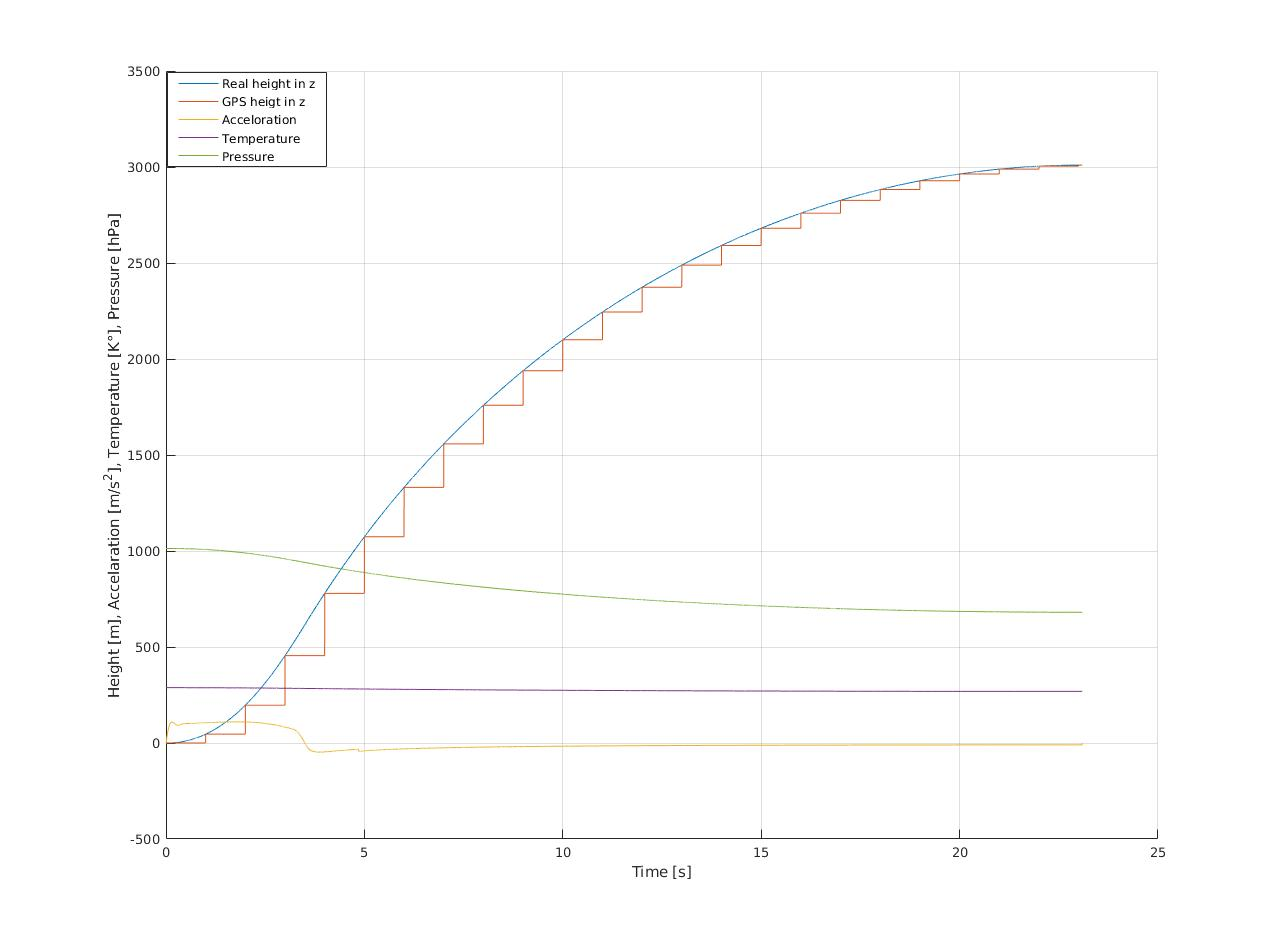
\includegraphics[width=\textwidth]{./Pictures/GeneratedSensorData.jpg}
 % GeneratedSensorData.jpg: 0x0 pixel, 300dpi, 0.00x0.00 cm, bb=
 \caption{Generated sensor data}
 \label{fig:GeneratedPerfectSensor}
\end{figure}

\subsection{Accelorometer}
Due to the fact that whole simulation works with discreet time stamps, the derivative of the height can not be done formally.
So it is done by calculating the difference in each data point to the next and then weight those by the delta in time between them.
This has to be done two times to get from the height to the acceleration.
The unit for the acceloration in this simulation is meter per second squared.

\subsection{Gyrometer}
As stated before the pitch angle can not be directly generated.
But if the  data from the test flights are visited. It can be seen that the angle stays more or less the same wile the motor is burning.
This make sense because during this time the main acceleration comes from one determinet direction and stabilices the rocket.
After the burnout the pitch angle does change more or less randomly depending on strength and direction of the wind that hits the rocket.
To reanimate this the values are generated randomly and the low pass filtered with a moving average filter to represent that behaviour.
While doing this the random values are kept small during the burning of the motor and exceed afterwards to higher values.

\subsection{Barometer}
The measurements from the barometer are depending on the formula stated in chapter \ref{ch:Approach}.
For reasons of simlicity the start pressure is choosen as the mean pressure at sea level which is 1013.35 hPa.
Also the temperature at the beginning is chosen as 288.15 degree Kelvin (15 degree Celcius) which also represents the mean value on the sea level.
At least the temperature gradient is - 0.0065 °/m which is a common used value.
For the state estimation in a test flight those values have to be determined before the start.

\subsection{GPS}
As stated in chapter \ref{ch:Approach} the GPS signal is just the height with a different sampling time. 
To maintain the vectors length which simplifies the later use in the estimation algorithm,
the signal is acquired with a zero order hold conversion instead of a down sampling. 

% Add code for the zero order Holde convertion

\subsection{Noise}
To generate the noise out of the data from the test flight, this has first to be extracted.
It is assumed that the noise on the data is different depending on the state of the rocket (before Icognition, during motor burning, after burnout till parachute ejection),
but it should have more or less the same properties between those events.
Depending on this, the data vector have first to be separated in those different sections.
For this the accelorometer measurements are iterated to find the time stamps on which those events happen like in figure bla.

%% picture of acceloration of z axis with icognition, burnout and parachute ejection are marked

If done so, polynoms are fitted on this measurements with the least squared error method.
Those polynoms represent the function which is assumed to be the noiseless data with possible offsets.
So if now the test flight data is subtracted by those polynomial curves which results in the noise without a mean.
From this point on this noise can be examined on its parameters, like the power density, the probability distribution and the variance figure bla.

%% pictue of autocorrelation, histogramm etc from sensor data noise

This noise data can now used tho solve the yule walker equation to get an AR-model.
But first, the data has to be resampled so that the AR-models can be used proper in the simulation.
With those AR-models, the noise can be regenerated by filtering white noise with the correct variance.
This generated noise can now be compared to the noise form the test flight data.

%% picture of pwelch plot from both noise vectors

As seen in figure bla those noise resemble each other in their power density spectrum much more the white noise would.
So the AR-model is exported to the simulation script an can there be used to generated the real sensor data.

\subsection{Accelorometer}
The noise which is on the accelorometer is special because it often has a drift which results in a more or less constant offset.
To recreate this, the offset can be estimated from the test flight data.
Especially the data before the icognition are help full, because the value that should be measured is known.

\subsection{Gyrometer}

\subsection{Barometer}
First there are two or more barometer which sample on different frequencies ant have therefore also different accuracies.
This is represented in the way that the variance of the noise from the slower sampled barometer is kept on a smaller value,
than that of the sensor which is faster sampled.


\subsection{GPS}
%The noise capacities of GPS is not real white. It more resembles a brown noise because it has a slow oscillation over it.
%I have to determine how i will remodel this in perticular.

\subsection{Real Sensor}
To now generated the real sensor data, the different noises have to be generated like stated above.
For this a vector of normal distributed random values is generated and multiplied by the square root of the corresponding variance.
This white noise is now filtered by the corresponding AR-model and can then be added onto the corresponding perfect sensor data.
This now results in the real sensor data.

\subsection{Accelorometer}
To generate the real acceleration data, in addition to the noise, also an offset has to be laied of it.


\subsection{Gyrometer}


\subsection{Barometer}


\subsection{GPS}



\section{State Estimator} %% Do this maybe in introduction because it is not specific to this simulation
As stated the used state estimator is a kalman filter with dynamic noises on the system as well as on the measurements.
This algorithm works in 4 main equations which can be devided into prediction and correction steps figure \ref{fig:Kalmanfilter}.

\begin{figure}[h!]
  \centering
  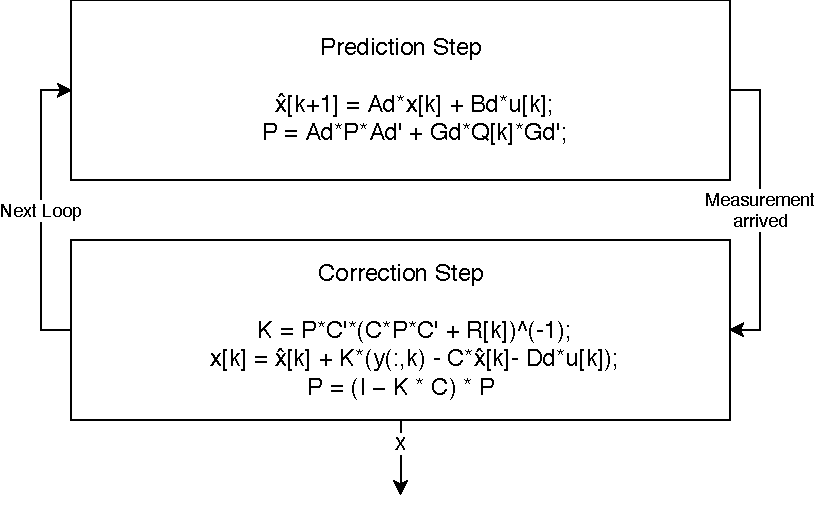
\includegraphics[width = \textwidth]{../BDADoku/Pictures/KalFIlFunc.pdf}
  \caption{Kalmanfilter}
  \label{fig:Kalmanfilter}
\end{figure}

\subsection{Prediction}
The prediction equations take the currently values of the state vector ($x[k]$)
and uses the time depending system model part (A) to predict the state values for the next time step $\hat{x}[k+1]$.
The hat denotes that this value is an assumption.
This with the equation: $$ \hat{x}[k+1] = AD*x[k] + Bd*u[k] $$
In addition the certainty matrix (P) is calculated which means that it is calculated how trustwotrhy those predictions are.
$$ P = Ad*P*Ad' + Gd*Q[k]*Gd'$$
For this the system noise is used, so with the help of the Q matrix it can be stated how well known the system is in this
time step.

\subsection{Correction Step}
If the measurements arrive those will be used can be used in the correction step to correct the prediction.
First the Kalmangain (K) is calculated with the equation.
$$ K = P*C'*(C*P*C' + R[k])^(-1) $$ 
This uses the P matrix from the prediction step as well as the R matrix which represents the measurments noise (how certain the values from the measurements are).
K is then used in the last equation $$x[k] = \hat{x}[k] + K*(y[k] - C*\hat{x}[k]-Dd*u[k])$$.
With this the measurement is used to correct the predicted value of the state vector with there uncertainties taken into account 

For this the matrices for the system models (A,B,C,D), the measurements noise (Q) as well as the system noises (R) have to be defined.

\section{System Model}
The models are modelled as stated in chapter \ref{ch:Approach} but from this different uses can be made out of this.
Due to this, these different implementation are tested and evaluated in the next chapter 

\section{Measurements noise}
The measurement noise matrix on each timestamp is veriliy easy to get in this simulation because the perfect measurememnts are known.
First the it can be just one variance per data vector be used to simplifie the whole process but this should not be to accurate.
As a second possibilties the varaince can be calcuated different for before and after burnout.
It can be assumed that this should be possible to measure in the real flights so it can be worked with those.


\section{System noises}
For the system noise the behavior of the system during the flight has to be examinated.



\subsection{Loop}
